\documentclass[aspectratio=169,11pt]{beamer}

\usepackage[T1]{fontenc}
\usepackage{graphicx}
\usepackage{amsmath}
\usepackage{amssymb}
\usepackage{mathrsfs}
\usepackage{tikz}
\usepackage{listings}
\usepackage{xcolor}
\usetikzlibrary{arrows.meta,positioning,calc,fit,backgrounds}

\usetheme{SEPOC2026}

% ==========================================================================
% Hide the theme's header / footer graphics.
% The SEPOC2026 theme draws a banner in the headline and a sponsor logo bar
% in the footline. Blanking the two templates removes those images; only a
% minimal page number is kept in the footline.
% NOTE: \usetheme must come BEFORE \logo{}, otherwise the theme overrides it.
% ==========================================================================
\setbeamertemplate{headline}{}
\setbeamertemplate{footline}{%
  \hfill\scriptsize\insertframenumber\,/\,\inserttotalframenumber\hspace*{2ex}\vspace*{1.2ex}%
}
\logo{}
% If part of the banner is painted on the background layer, uncomment:
% \setbeamertemplate{background canvas}{}
% \setbeamertemplate{background}{}

% --------------------------------------------------------------------------
% Frame titles: keep the theme's title font, but pin the title 3mm from the
% paper edge instead of the theme's wide left pad, and give it a light orange
% accent (orange title text, no rule underneath).
% To borrow the theme's own accent instead of this orange, replace
% \color{tkaccent} by \usebeamercolor[fg]{structure} below.
% Comment the whole block out to restore the original theme title style.
% --------------------------------------------------------------------------
\definecolor{tkaccent}{HTML}{E8730C}
\makeatletter
\setbeamertemplate{frametitle}{%
  \vskip0.4ex%
  \noindent\hspace*{\dimexpr 3mm-\beamer@leftmargin\relax}%
  \hbox to \dimexpr\textwidth+\beamer@leftmargin-3mm\relax{%
    \usebeamerfont{frametitle}\color{tkaccent}\insertframetitle\hfil}%
  \vskip-0.2ex%
}
\makeatother

% ============================================================ macros
\newcommand{\bz}{\mathbf{0}}
\newcommand{\bo}{\mathbf{1}}
\newcommand{\rk}{k}
% The rule names of the paper, kept verbatim so that the slides can be read
% side by side with the article. \ensuremath lets them be used in text too.
\newcommand{\Rer}{\ensuremath{\mathscr{R}^{r}_{er}}}
\newcommand{\Rgo}{\ensuremath{\mathscr{R}^{r}_{go}}}
\newcommand{\RvEr}{\ensuremath{\mathscr{R}_{er}}}
\newcommand{\Rreset}{\ensuremath{\mathscr{R}_{reset}}}
\newcommand{\RerRank}{\ensuremath{\mathscr{R}_{erRank}}}
\newcommand{\Rjoin}{\ensuremath{\mathscr{R}_{join}}}
\newcommand{\Rtok}{\ensuremath{\mathscr{R}_{tok}}}
\newcommand{\Radd}{\ensuremath{\mathscr{R}_{add}}}
\newcommand{\Rready}{\ensuremath{\mathscr{R}_{ready}}}
% A (k,t,b) triple that CHANGED with respect to the previous round: red and
% bold. \boldmath must be issued in text mode, before the math shift.
\newcommand{\trC}[1]{{\boldmath\color{red}#1}}

% ==========================================================================
% ONE text size for every bullet list of the deck, and ONE size for every
% caption under a figure. Never set the size of a bullet list locally: use
% \bodyfont, so that all ten frames stay visually identical.
% ==========================================================================
\newcommand{\bodyfont}{\footnotesize}
\newcommand{\captionfont}{\fontsize{7.5}{9.0}\selectfont}
% The theme sets the text of a nested list to a fixed size, which is larger
% than the \bodyfont of the list that contains it, so a sub-item could come
% out bigger than its own item. Pin every depth to \bodyfont: the indentation
% already shows the nesting, so the size must not change with the depth.
\setbeamerfont{itemize/enumerate body}{size=\bodyfont}
\setbeamerfont{itemize/enumerate subbody}{size=\bodyfont}
\setbeamerfont{itemize/enumerate subsubbody}{size=\bodyfont}

% ============================================================ tikz styles
\tikzset{
  gnode/.style={circle,draw,thick,inner sep=0pt,minimum size=5.6mm,font=\scriptsize},
  groot/.style={rectangle,draw,thick,inner sep=1pt,minimum size=5.6mm,font=\scriptsize},
  rnode/.style={circle,draw,thick,dashed,inner sep=0pt,minimum size=5.6mm,font=\scriptsize},
  gedge/.style={thick,draw=gray!70},
  garr/.style={-{Stealth[length=1.7mm]},thick,draw=teal!80!black},
  lbl/.style={font=\tiny,inner sep=1pt},
  clbl/.style={font=\scriptsize,inner sep=1pt}
}
% Enlarged label font for the small explanatory graphs of the root slide.
% Used as an option of a tikzpicture: [scale=...,transform shape,bigtext]
\tikzset{bigtext/.style={%
  gnode/.append style={font=\small},
  groot/.append style={font=\small},
  rnode/.append style={font=\small},
  clbl/.append  style={font=\small}}}
% --- annotated local-state tree of the "local variables" slide ---
% Each circle shows \rk_v (or \top / \bot for the error / reset node);
% the (k,t,b) triple of the node is written just to its right.
\tikzset{
  stnode/.style={circle,draw,thick,inner sep=0pt,minimum size=5.0mm,%
                 font=\fontsize{5.2}{5.8}\selectfont},
  stroot/.style={stnode,rectangle},
  stlbl/.style={font=\fontsize{5.0}{6.0}\selectfont,inner sep=0.6pt,%
                anchor=center,fill=white},
  stdead/.style={thick,dashed,draw=gray!65}
}
% --- a yellow "TOKEN" tag on the top-right corner of a node means: token held
% Used by the "algorithm overview" slide, where the same chain is drawn at
% five consecutive rounds, so the only changing marks are t, b and the tag.
\tikzset{
  ttok/.style={draw=black,line width=0.3pt,fill=yellow,text=black,
               font=\fontsize{4.4}{5.0}\selectfont\bfseries,
               inner sep=0.9pt,rounded corners=0.4pt},
  % (k,t,b) triple placed above a node: one step larger than \stlbl
  trip/.style={font=\fontsize{6.4}{7.4}\selectfont,inner sep=0.5pt,%
               anchor=center,fill=white},
  % one-line caption under one round of the same figure
  capt/.style={font=\fontsize{5.2}{6.2}\selectfont,inner sep=0.4pt,align=left}
}
% --- twice the size of \lbl, for the rule labels of the state automaton ---
\tikzset{rlbl/.style={font=\fontsize{12}{14}\selectfont,inner sep=1pt}}
% ============================================================ rank colour code
% ONE colour code for every graph of the deck: the fill of a node encodes its
% rank and nothing else.
%   0 -> blue, 1 -> green, 2 -> orange,
%   an error state (b = top) -> red, a reset state (k = bot) -> gray,
%   a node whose rank is unknown / parametric -> white with a black frame.
% Node text is 0/1/2/bot/top; a node name (u1, v, r, ...) goes beside the
% node and a (k,t,b) triple, when needed, goes above it.
\tikzset{
  c0/.style={fill=blue!20},
  c1/.style={fill=green!25},
  c2/.style={fill=orange!30},
  cE/.style={fill=red!22},
  cR/.style={fill=gray!18},
  cX/.style={fill=white}
}
% ============================================================ JS listings
\lstdefinestyle{js}{
  language=Java,
  basicstyle=\ttfamily\tiny,
  keywordstyle=\color{blue!70!black}\bfseries,
  commentstyle=\color{green!45!black}\itshape,
  stringstyle=\color{red!60!black},
  frame=single,
  framesep=3pt,
  rulecolor=\color{gray!45},
  breaklines=true,
  columns=fullflexible,
  keepspaces=true,
  showstringspaces=false,
  aboveskip=2pt,
  belowskip=2pt,
  xleftmargin=2pt,
  xrightmargin=2pt,
  morekeywords={function,const,let,if,else,return,true,false,null,undefined}
}
\lstset{style=js}

% Tighter variant used in the math || JavaScript frames: smaller font, no
% extra space above/below the frame and no side margins, so the code column
% can be widened and pushed up to the top of the slide.
\lstdefinestyle{jsc}{
  style=js,
  basicstyle=\ttfamily\fontsize{5.1}{5.7}\selectfont,
  aboveskip=0pt,
  belowskip=0pt,
  framesep=2pt,
  xleftmargin=4mm,   % pushes the frame to the right, away from the math column
  xrightmargin=0pt
}

% ============================================================ metadata
\title[TokBin]{Deterministic Synchronous Self-Stabilizing BFS Construction with Constant Space Complexity}
\subtitle{A rule-by-rule walk-through of \texttt{TokBin}}
\author{L\'elia Blin \and Franck Petit \and S\'ebastien Tixeuil}
\date{}

\begin{document}

% ==========================================================================
% 1 -- TITLE
% ==========================================================================
\begin{frame}
  % Title page in the deck's accent colour (tkaccent, defined above).
  \setbeamercolor{title}{fg=tkaccent}
  \setbeamercolor{subtitle}{fg=tkaccent!80!black}
  \setbeamercolor{author}{fg=black!85}
  \setbeamercolor{institute}{fg=black!70}
  % Accent rule under the main title (title page only).
  \setbeamertemplate{title}{%
    \usebeamerfont{title}\usebeamercolor[fg]{title}\inserttitle\par
    \vspace{0.3ex}%
    {\color{tkaccent}\rule{\linewidth}{0.9pt}}\par
    \vspace{-0.3ex}%
  }
  \titlepage
  \vspace*{-3mm}
  \begin{center}
    {\scriptsize Presentation: CHE CHON HONG, University of Macau}
  \end{center}
\end{frame}

% ==========================================================================
% 2 -- MODEL AND PROBLEM
% ==========================================================================
\begin{frame}{Model and Problem}
\centering
\vspace*{-2mm}
% One graph, two copies of the SAME 20-node graph at the SAME coordinates:
%   left  = the input, an anonymous connected undirected graph, no rank shown,
%           and with extra chords that the BFS tree does NOT use;
%   right = the same graph once the protocol has stabilised to BFS^{=3}.
% The arrow in between stands for the computation itself.
% NB: the horizontal shift of the second copy MUST carry a unit -- a bare
% number is interpreted in points by pgfmath, which made the two graphs
% overlap. A coordinate in the shift key is in the graph unit (cm).
\resizebox{0.88\textwidth}{!}{%
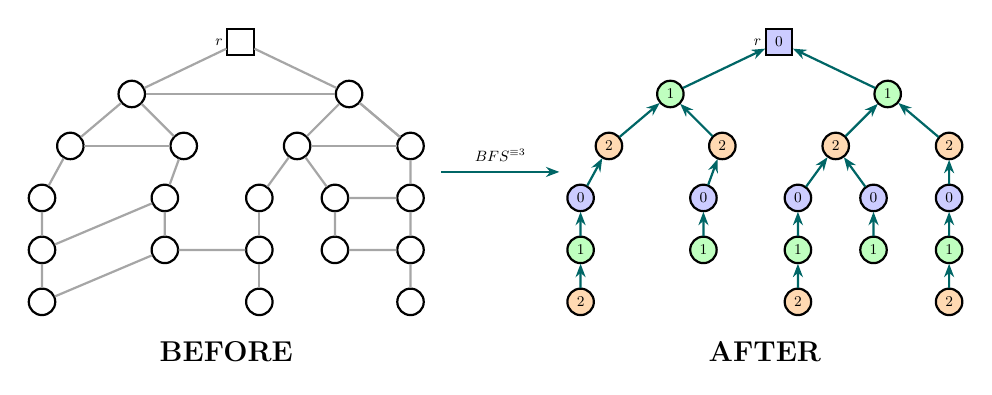
\begin{tikzpicture}[scale=0.60,transform shape,bigtext]
  % -------------------------------------------------- left: the input graph
  \node[groot] (ar)  at ( 0.0, 0.00){};
  \node[clbl,left=0.4mm of ar] {$r$};
  \node[gnode] (au1)  at (-2.3,-1.10){};
  \node[gnode] (au2)  at ( 2.3,-1.10){};
  \node[gnode] (au3)  at (-3.6,-2.20){};
  \node[gnode] (au4)  at (-1.2,-2.20){};
  \node[gnode] (au5)  at ( 1.2,-2.20){};
  \node[gnode] (au6)  at ( 3.6,-2.20){};
  \node[gnode] (au7)  at (-4.2,-3.30){};
  \node[gnode] (au8)  at (-1.6,-3.30){};
  \node[gnode] (au9)  at ( 0.4,-3.30){};
  \node[gnode] (au10) at ( 2.0,-3.30){};
  \node[gnode] (au11) at ( 3.6,-3.30){};
  \node[gnode] (au12) at (-4.2,-4.40){};
  \node[gnode] (au13) at (-1.6,-4.40){};
  \node[gnode] (au14) at ( 0.4,-4.40){};
  \node[gnode] (au15) at ( 2.0,-4.40){};
  \node[gnode] (au16) at ( 3.6,-4.40){};
  \node[gnode] (au17) at (-4.2,-5.50){};
  \node[gnode] (au18) at ( 0.4,-5.50){};
  \node[gnode] (au19) at ( 3.6,-5.50){};
  % the edges of the BFS tree -- undirected, no orientation, no rank
  \draw[gedge] (au1)--(ar);   \draw[gedge] (au2)--(ar);
  \draw[gedge] (au3)--(au1);  \draw[gedge] (au4)--(au1);
  \draw[gedge] (au5)--(au2);  \draw[gedge] (au6)--(au2);
  \draw[gedge] (au7)--(au3);  \draw[gedge] (au8)--(au4);
  \draw[gedge] (au9)--(au5);  \draw[gedge] (au10)--(au5);
  \draw[gedge] (au11)--(au6);
  \draw[gedge] (au12)--(au7); \draw[gedge] (au13)--(au8);
  \draw[gedge] (au14)--(au9); \draw[gedge] (au15)--(au10);
  \draw[gedge] (au16)--(au11);
  \draw[gedge] (au17)--(au12); \draw[gedge] (au18)--(au14);
  \draw[gedge] (au19)--(au16);
  % extra chords of the input graph, absent from the BFS tree; every one of
  % them joins two nodes whose BFS levels differ by at most one, so none of
  % them changes a distance -- the right-hand graph is still the BFS answer.
  \draw[gedge] (au1)--(au2);   \draw[gedge] (au3)--(au4);
  \draw[gedge] (au5)--(au6);   \draw[gedge] (au2)--(au6);
  \draw[gedge] (au10)--(au11); \draw[gedge] (au13)--(au14);
  \draw[gedge] (au15)--(au16); \draw[gedge] (au12)--(au8);
  \draw[gedge] (au17)--(au13);
  % ------------------------------------------------ right: the BFS output
  \begin{scope}[shift={(11.4,0)}]
  \node[groot,c0] (br)  at ( 0.0, 0.00){$0$};
  \node[clbl,left=0.4mm of br] {$r$};
  \node[gnode,c1] (bu1)  at (-2.3,-1.10){$1$};
  \node[gnode,c1] (bu2)  at ( 2.3,-1.10){$1$};
  \node[gnode,c2] (bu3)  at (-3.6,-2.20){$2$};
  \node[gnode,c2] (bu4)  at (-1.2,-2.20){$2$};
  \node[gnode,c2] (bu5)  at ( 1.2,-2.20){$2$};
  \node[gnode,c2] (bu6)  at ( 3.6,-2.20){$2$};
  \node[gnode,c0] (bu7)  at (-4.2,-3.30){$0$};
  \node[gnode,c0] (bu8)  at (-1.6,-3.30){$0$};
  \node[gnode,c0] (bu9)  at ( 0.4,-3.30){$0$};
  \node[gnode,c0] (bu10) at ( 2.0,-3.30){$0$};
  \node[gnode,c0] (bu11) at ( 3.6,-3.30){$0$};
  \node[gnode,c1] (bu12) at (-4.2,-4.40){$1$};
  \node[gnode,c1] (bu13) at (-1.6,-4.40){$1$};
  \node[gnode,c1] (bu14) at ( 0.4,-4.40){$1$};
  \node[gnode,c1] (bu15) at ( 2.0,-4.40){$1$};
  \node[gnode,c1] (bu16) at ( 3.6,-4.40){$1$};
  \node[gnode,c2] (bu17) at (-4.2,-5.50){$2$};
  \node[gnode,c2] (bu18) at ( 0.4,-5.50){$2$};
  \node[gnode,c2] (bu19) at ( 3.6,-5.50){$2$};
  % every edge points towards the parent of the BFS tree
  \draw[garr] (bu1)--(br);   \draw[garr] (bu2)--(br);
  \draw[garr] (bu3)--(bu1);  \draw[garr] (bu4)--(bu1);
  \draw[garr] (bu5)--(bu2);  \draw[garr] (bu6)--(bu2);
  \draw[garr] (bu7)--(bu3);  \draw[garr] (bu8)--(bu4);
  \draw[garr] (bu9)--(bu5);  \draw[garr] (bu10)--(bu5);
  \draw[garr] (bu11)--(bu6);
  \draw[garr] (bu12)--(bu7); \draw[garr] (bu13)--(bu8);
  \draw[garr] (bu14)--(bu9); \draw[garr] (bu15)--(bu10);
  \draw[garr] (bu16)--(bu11);
  \draw[garr] (bu17)--(bu12); \draw[garr] (bu18)--(bu14);
  \draw[garr] (bu19)--(bu16);
  \end{scope}
  % ------------------------------------------------ the computation itself
  \draw[garr] (4.25,-2.75) -- (6.75,-2.75);
  \node[font=\small,above=0.9mm] at (5.50,-2.75) {$BFS^{\equiv 3}$};
  % captions of the two halves
  \node[font=\fontsize{16}{18}\selectfont\bfseries] at (-0.3,-6.55) {BEFORE};
  \node[font=\fontsize{16}{18}\selectfont\bfseries] at (11.1,-6.55) {AFTER};
\end{tikzpicture}}

\vspace{1mm}
{\bodyfont
\begin{columns}[T]
\begin{column}{0.47\textwidth}
\begin{itemize}\setlength\itemsep{2pt}
\item Connected, undirected, anonymous
\item \textbf{Semi-uniform}: one distinguished root
\item No global parameters: $n$ / $\Delta$ / $\varepsilon$
\end{itemize}
\end{column}
\begin{column}{0.50\textwidth}
\begin{itemize}\setlength\itemsep{2pt}
\item \textbf{Goal: BFS} --- the distance to the root, modulo 3
\item Constant space --- 6 bits per node, at any size
\item Deterministic, synchronous, self-stabilizing from any state
\end{itemize}
\end{column}
\end{columns}}
\end{frame}

% ==========================================================================
% 3 -- MOTIVATION: PAST WORK AND DIFFICULTY
% ==========================================================================
\begin{frame}{Why is this problem hard?}
\bodyfont
\begin{columns}[T]
\begin{column}{0.48\textwidth}
\textbf{Space--time trade-off}
\begin{itemize}\setlength\itemsep{5pt}
\item silent $\Rightarrow$ $\Omega(\log n)$ bits
\item talkative $\Rightarrow$ $O(\log\log n+\log\Delta)$ bits
\item constant space only with pointers
\item no leader $\Rightarrow$ impossible
\end{itemize}
\end{column}
\begin{column}{0.48\textwidth}
\textbf{Why constant space is hard}
\begin{itemize}\setlength\itemsep{5pt}
\item \textbf{anonymous}: cannot name a parent
\item \textbf{no counter}: cannot detect a cycle
\item a moving token stays in the loop forever
\item any stored pointer breaks the $O(1)$ bound
\end{itemize}
\end{column}
\end{columns}

% the answer to both columns, centred at the foot of the slide in a
% bordered box so it reads as the conclusion of the frame
\vfill
\begin{center}

\begin{tikzpicture}
  \node[draw=tkaccent,line width=0.9pt,rounded corners=2pt,
        fill=tkaccent!8,inner sep=4.2pt,font=\small]
    {\textbf{Our idea:} one token whose lifespan is bounded};
\end{tikzpicture}
\end{center}
\vspace{1mm}
\end{frame}

% ==========================================================================
% 4 -- ALGORITHM OVERVIEW / TOKEN FLOW
% ==========================================================================
\begin{frame}{Algorithm Overview}
\vspace*{-3mm}
\begin{columns}[T]
\begin{column}{0.44\textwidth}
\bodyfont
% The bullet list owns most of the left column, so its list margins are pulled
% in: \leftmargini shrinks the bullet indent (default 2.5em at 11pt) and a
% negative \rightmargin lets the text run a little past the column, into the
% 0.02\textwidth gutter between the columns. Net gain is about 2em per line.
\setlength{\leftmargini}{1.2em}
\setlength{\rightmargin}{-0.6em}
\begin{itemize}\setlength\itemsep{6pt}
\item Two programs:
  \begin{itemize}\setlength\itemsep{1pt}
  \item $\mathtt{tokbinR}$ at the root
  \item $\mathtt{tokbinV}$ at all other nodes
  \end{itemize}
\item Root sends tokens; duplicates \textbf{merge}
\item One \emph{bit} per node, flipped on every arrival
\item Sends a token only if the next neighbour's bit allows
\item Bounded lifespan $\Rightarrow$ no cycle keeps a token forever
\item Stabilizes in $O(2^{\varepsilon})$ rounds; never silent
\end{itemize}
\end{column}
\begin{column}{0.54\textwidth}
\centering
% ---- the smallest possible round: one root, two children -------------
% The parent links point up (child -> root), exactly as everywhere else in
% the deck; the two orange arcs are the tokens themselves, going DOWN one
% level, which is the only thing this slide has to convey.
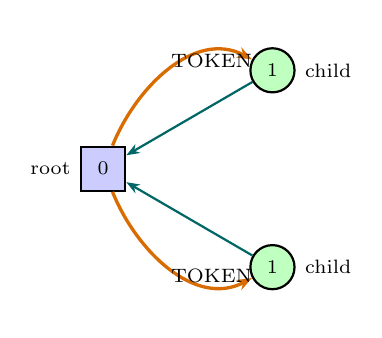
\begin{tikzpicture}[scale=1.0,transform shape]
  \node[groot,c0] (r) at (0,0) {$0$};
  \node[clbl,left=0.8mm of r] {root};
  \node[gnode,c1] (a) at (2.15, 1.25) {$1$};
  \node[gnode,c1] (b) at (2.15,-1.25) {$1$};
  \node[clbl,right=0.8mm of a] {child};
  \node[clbl,right=0.8mm of b] {child};
  \draw[garr] (a)--(r);
  \draw[garr] (b)--(r);
  % the token leaves the root and goes down to BOTH children; the two arcs
  % bow outwards so they never sit on top of the parent links
  \draw[-{Stealth[length=1.9mm]},very thick,draw=orange!85!black]
    (r) to[out=68,in=152]
    node[midway,above right=-0.6mm,font=\scriptsize,inner sep=1pt]{TOKEN} (a);
  \draw[-{Stealth[length=1.9mm]},very thick,draw=orange!85!black]
    (r) to[out=-68,in=-152]
    node[midway,below right=-0.6mm,font=\scriptsize,inner sep=1pt]{TOKEN} (b);
\end{tikzpicture}
\par\vspace{2mm}
{\captionfont The root sends one token down to every child.}
\end{column}
\end{columns}
\end{frame}

% ==========================================================================
% 5 -- VISUALIZATION
% ==========================================================================
\begin{frame}{Visualization}
\centering
\vspace*{-2mm}
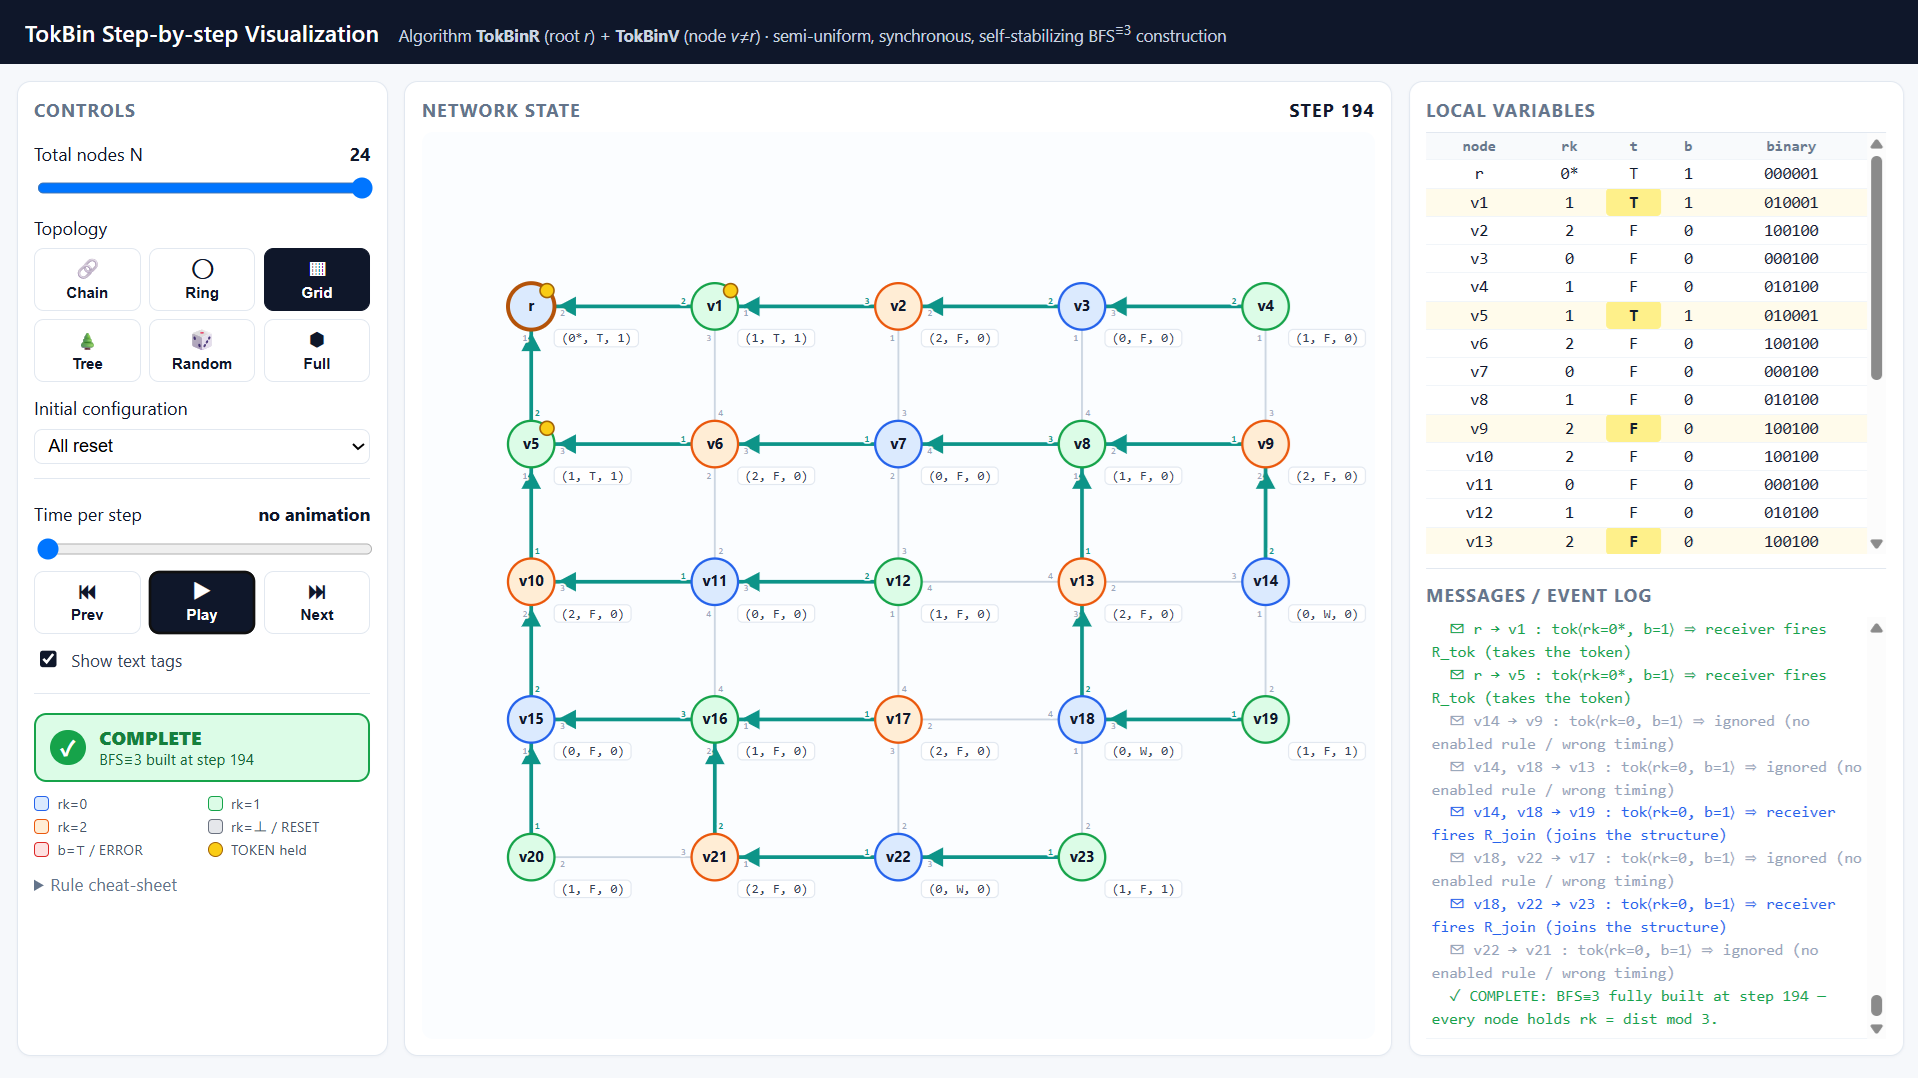
\includegraphics[height=0.70\textheight,width=\textwidth,keepaspectratio]{tokbin-sim.png}

\vspace{1.5mm}
{\bodyfont
 \href{https://jasonisgood.online/um/tokbin.html}%
      {\color{blue}\underline{Live demo}}}
\end{frame}

% ==========================================================================
% 6 -- LOCAL VARIABLES AND STATE SPACE
% ==========================================================================
\begin{frame}{Local variables}
\begin{columns}[T]
\begin{column}{0.55\textwidth}
\bodyfont
\begin{itemize}\setlength\itemsep{4pt}
\item \textbf{Three variables} per node
  \begin{itemize}\setlength\itemsep{1pt}
  \item $\rk$: $0/1/2/\bot$ --- distance mod 3; $\bot$ = reset
  \item $t$: $\mathrm{FALSE}$, $\mathrm{TRUE}$, or $\mathrm{WAIT}$
  \item $b$: $0$, $1$, or $\top$ = error
  \end{itemize}
\item \textbf{State space} $4\times3\times3=36$
\item \textbf{Memory} 6 bits $=O(1)$
\item \textbf{Example} $(2,\mathrm{TRUE},\bo)\mapsto\mathtt{10\,01\,01}$
\end{itemize}
\end{column}
\begin{column}{0.45\textwidth}
\centering
\vspace*{-1mm}
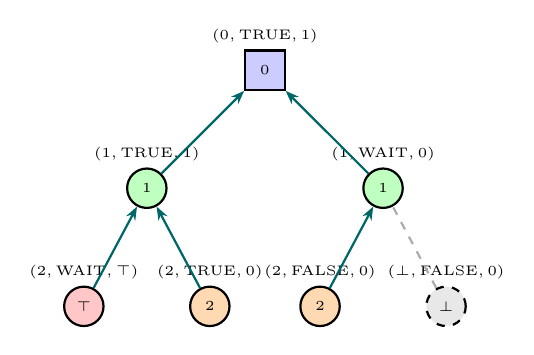
\begin{tikzpicture}
  % ---- one snapshot: 7 nodes, depth 2, one error node, one reset node ----
  % root (k = 0) -> two children (k = 1) -> two sub-children each (k = 2);
  % one of the four carries an error, one of them is reset
  \node[stroot,c0]      (r) at (2.400, 0.00) {$0$};
  \node[stlbl,above=0.5mm of r] {$(0,\mathrm{TRUE},1)$};
  \node[stnode,c1]      (a) at (0.900,-1.50) {$1$};
  \node[stlbl,above=0.5mm of a] {$(1,\mathrm{TRUE},1)$};
  \node[stnode,c1]      (b) at (3.900,-1.50) {$1$};
  \node[stlbl,above=0.5mm of b] {$(1,\mathrm{WAIT},0)$};
  \node[stnode,cE]      (d) at (0.100,-3.00) {$\top$};
  \node[stlbl,above=0.5mm of d] {$(2,\mathrm{WAIT},\top)$};
  \node[stnode,c2]      (e) at (1.700,-3.00) {$2$};
  \node[stlbl,above=0.5mm of e] {$(2,\mathrm{TRUE},0)$};
  \node[stnode,c2]      (f) at (3.100,-3.00) {$2$};
  \node[stlbl,above=0.5mm of f] {$(2,\mathrm{FALSE},0)$};
  \node[stnode,dashed,cR] (g) at (4.700,-3.00) {$\bot$};
  \node[stlbl,above=0.5mm of g] {$(\bot,\mathrm{FALSE},0)$};
  % ---- an arrow means: this edge is a legal parent link -----------
  \draw[garr]   (a)--(r);  \draw[garr] (b)--(r);
  \draw[garr]   (d)--(a);  \draw[garr] (e)--(a);
  \draw[garr]   (f)--(b);
  \draw[stdead] (g)--(b);
\end{tikzpicture}

\vspace{1.5mm}
{\captionfont Example: nodes with different $(k,t,b)$.}
\end{column}
\end{columns}
\end{frame}

% ==========================================================================
% 7 -- KINSHIP AND RESET
% ==========================================================================
\begin{frame}{Kinship structure}
% three text blocks, left to right: family / reset / parent choice.
% Equal widths, list indentation cut to a minimum so that the short lines of
% each block do not wrap.
\noindent
\begin{columns}[T,totalwidth=\textwidth]
\begin{column}{0.325\textwidth}
\bodyfont
\setlength{\leftmargini}{0.6em}
\setlength{\leftmarginii}{0.6em}
\setlength{\parindent}{0pt}
\begin{itemize}\setlength\itemsep{3pt}\setlength{\parsep}{0pt}
\item \textbf{Family}: rank mod 3
  \begin{itemize}\setlength\itemsep{1pt}\setlength{\parsep}{0pt}
  \item parent: $\rk-1$
  \item child: $\rk+1$
  \item sibling: $\rk$
  \end{itemize}
\end{itemize}
\end{column}
\begin{column}{0.325\textwidth}
\bodyfont
\setlength{\leftmargini}{0.6em}
\setlength{\leftmarginii}{0.6em}
\setlength{\parindent}{0pt}
\begin{itemize}\setlength\itemsep{3pt}\setlength{\parsep}{0pt}
\item \textbf{Reset} $\rk=\bot$
  \begin{itemize}\setlength\itemsep{1pt}\setlength{\parsep}{0pt}
  \item no family
  \item ignores every token
  \end{itemize}
\end{itemize}
\end{column}
\begin{column}{0.325\textwidth}
\bodyfont
\setlength{\leftmargini}{0.6em}
\setlength{\leftmarginii}{0.6em}
\setlength{\parindent}{0pt}
\begin{itemize}\setlength\itemsep{3pt}\setlength{\parsep}{0pt}
\item \textbf{Parent choice}
  \begin{itemize}\setlength\itemsep{1pt}\setlength{\parsep}{0pt}
  \item smallest port number
  \item among $\rk-1$ neighbours
  \end{itemize}
\end{itemize}
\end{column}
\end{columns}

\vspace{3mm}
% three small graphs side by side, left to right
\begin{center}
% ---- (1) kinship: the family sets are read off the ranks ----------
\begin{minipage}[t]{0.32\linewidth}
\centering
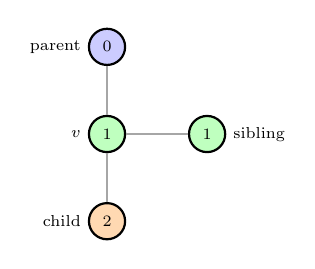
\begin{tikzpicture}[scale=0.82,transform shape]
  \node[gnode,c0] (p) at (0, 1.35) {$0$};
  \node[gnode,c1] (v) at (0, 0)    {$1$};
  \node[gnode,c2] (c) at (0,-1.35) {$2$};
  \node[gnode,c1] (s) at (1.55,0)  {$1$};
  \draw[gedge] (p)--(v);
  \draw[gedge] (v)--(c);
  \draw[gedge] (v)--(s);
  \node[clbl,left=0.7mm of p] {parent};
  \node[clbl,left=0.7mm of v] {$v$};
  \node[clbl,left=0.7mm of c] {child};
  \node[clbl,right=0.7mm of s] {sibling};
\end{tikzpicture}
\\[1mm]{\captionfont (1) family}
\end{minipage}\hfill
% ---- (2) reset state: a dormant node ignores every token ---------
\begin{minipage}[t]{0.32\linewidth}
\centering
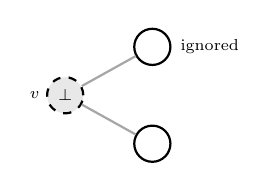
\begin{tikzpicture}[scale=0.82,transform shape]
  \node[rnode,cR] (x) at (0,0) {$\bot$};
  \node[clbl,left=0.6mm of x] {$v$};
  \node[gnode,cX] (n1) at (1.35,0.75) {};
  \node[gnode,cX] (n2) at (1.35,-0.75) {};
  \draw[gedge] (x)--(n1); \draw[gedge] (x)--(n2);
  \node[clbl,right=1mm of n1] {ignored};
\end{tikzpicture}
\\[1mm]{\captionfont (2) reset: no family}
\end{minipage}\hfill
% ---- (3) parent selection: the smallest port wins ---------------
\begin{minipage}[t]{0.32\linewidth}
\centering
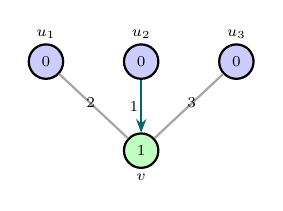
\begin{tikzpicture}[scale=0.78,transform shape]
  \node[gnode,c0] (u1) at (-1.55,0.9) {$0$};
  \node[gnode,c0] (u2) at ( 0.00,0.9) {$0$};
  \node[gnode,c0] (u3) at ( 1.55,0.9) {$0$};
  \node[gnode,c1] (v)  at (0,-0.55)   {$1$};
  \node[clbl,above=0.4mm of u1] {$u_1$};
  \node[clbl,above=0.4mm of u2] {$u_2$};
  \node[clbl,above=0.4mm of u3] {$u_3$};
  \node[clbl,below=0.4mm of v] {$v$};
  \draw[gedge] (u1)--(v) node[midway,clbl,above left=-1mm]{$2$};
  \draw[garr]  (u2)--(v) node[midway,clbl,left=0mm]{$1$};
  \draw[gedge] (u3)--(v) node[midway,clbl,above right=-1mm]{$3$};
\end{tikzpicture}
\\[1mm]{\captionfont (3) ports $1,2,3$: $u_2$ wins}
\end{minipage}
\end{center}
\end{frame}

% ==========================================================================
% 8 -- ROOT ALGORITHM
% ==========================================================================
\begin{frame}{Root algorithm \texorpdfstring{$\mathtt{TokBinR}$}{TokBinR}}
\begin{columns}[T]
\begin{column}{0.53\textwidth}
\bodyfont
\textbf{Sees its whole neighbourhood}
\begin{itemize}\setlength\itemsep{3pt}
\item \textbf{synchronized}: all neighbours at rank 1,
      same $t$ and same $b$
\item \textbf{reset}: every neighbour is reset
\item \textbf{error}: every neighbour carries $\top$
\end{itemize}
\vspace{2.5mm}
\textbf{Two rules}
\begin{itemize}\setlength\itemsep{4pt}
\item \Rer: no condition holds $\rightarrow$ raise $\top$
\item \Rgo: all neighbours $\top$ $\rightarrow$ clear $\top$, restart
\end{itemize}
\end{column}
\begin{column}{0.44\textwidth}
\centering
\vspace*{6mm}
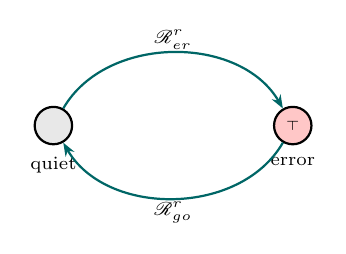
\begin{tikzpicture}[scale=0.95,transform shape,every node/.style={font=\scriptsize}]
  \node[stnode,cR] (Q) at (0,0)     {};
  \node[clbl,below=1.2mm of Q] {quiet};
  \node[stnode,cE] (E) at (3.2,0)   {$\top$};
  \node[clbl,below=1.2mm of E] {error};
  \draw[garr] (Q) to[out=60,in=120]  node[clbl,above]{\Rer} (E);
  \draw[garr] (E) to[out=-120,in=-60] node[clbl,below]{\Rgo} (Q);
\end{tikzpicture}
\par\vspace{2mm}
{\captionfont Algorithm $\mathtt{TokBinR}$}
\end{column}
\end{columns}
\end{frame}

% ==========================================================================
% 9 -- TOKBINV RULES
% ==========================================================================
\begin{frame}{Non-root algorithm \texorpdfstring{$\mathtt{TokBinV}$}{TokBinV}}
\vspace*{-2mm}
% exact halves, no stray indentation: \noindent plus zero list margins keeps
% the automaton centred inside the right half instead of drifting right
\noindent
\begin{columns}[T,totalwidth=\textwidth]
\begin{column}{0.40\textwidth}
\bodyfont
\setlength{\leftmargini}{0.6em}
\setlength{\leftmarginii}{0.6em}
\setlength{\rightmargin}{0pt}
\setlength{\parindent}{0pt}
\textbf{Seven rules}
\begin{itemize}\setlength\itemsep{7pt}\setlength{\topsep}{0pt}\setlength{\parsep}{0pt}
\item \RvEr: error nearby $\rightarrow$ raise $\top$
\item \Rreset: $\top$ or stale error $\rightarrow$ forget all
\item \RerRank: non-parent token $\rightarrow$ keep rank, $\top$
\item \Rjoin: dormant, reset parent $\rightarrow$ join it
\item \Rtok: a parent's token $\rightarrow$ take it
\item \Radd: holding it $\rightarrow$ pass on, flip $b$
\item \Rready: done $\rightarrow$ release, go quiet
\end{itemize}
\end{column}
\begin{column}{0.60\textwidth}
\centering
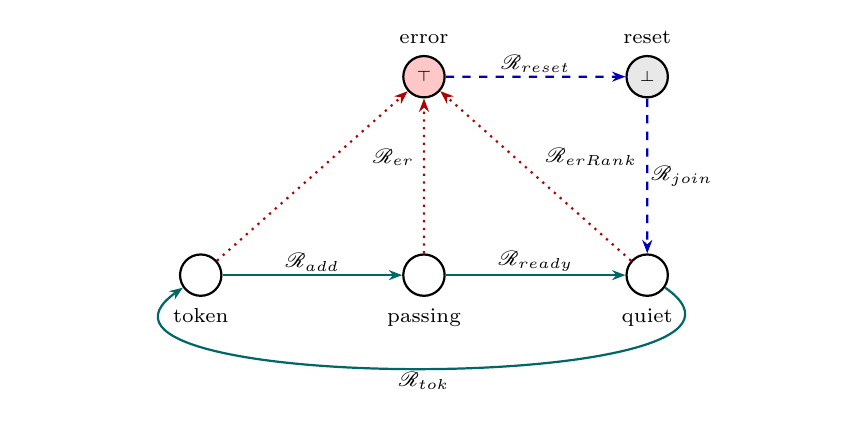
\begin{tikzpicture}[scale=1.05,transform shape,every node/.style={font=\scriptsize}]
  \node[stnode,cX] (A) at (0.0,0.0) {};
  \node[stnode,cX] (B) at (2.70,0.0) {};
  \node[stnode,cX] (C) at (5.40,0.0) {};
  \node[stnode,cE] (E) at (2.70,2.40) {$\top$};
  \node[stnode,cR] (R) at (5.40,2.40) {$\bot$};
  \node[clbl,below=1.0mm of A] {token};
  \node[clbl,below=1.0mm of B] {passing};
  \node[clbl,below=1.0mm of C] {quiet};
  \node[clbl,above=1.0mm of E] {error};
  \node[clbl,above=1.0mm of R] {reset};
  \draw[garr] (A)--node[clbl,above]{\Radd}(B);
  \draw[garr] (B)--node[clbl,above]{\Rready}(C);
  \draw[garr] (C) to[out=-35,in=-145] node[clbl,below]{\Rtok}(A);
  \draw[garr,dotted,draw=red!70!black] (A)--(E);
  \draw[garr,dotted,draw=red!70!black]
      (B)--node[clbl,above left=1.0mm]{\RvEr}(E);
  \draw[garr,dotted,draw=red!70!black]
      (C)--node[clbl,above right=1.0mm]{\RerRank}(E);
  \draw[garr,dashed,draw=blue!70!black] (E)--node[clbl,above]{\Rreset}(R);
  \draw[garr,dashed,draw=blue!70!black] (R)--node[clbl,right]{\Rjoin}(C);
\end{tikzpicture}
\par\vspace{2mm}
{\captionfont Algorithm $\mathtt{TokBinV}$}
\end{column}
\end{columns}
\end{frame}

% ==========================================================================
% 10 -- ERROR DETECTION (OVERVIEW)
% ==========================================================================
\begin{frame}{Error detection}
\begin{columns}[T]
\begin{column}{0.60\textwidth}
\bodyfont
\begin{itemize}\setlength\itemsep{3pt}
\item \textbf{Three kinds of error}
  \begin{itemize}\setlength\itemsep{1pt}
  \item \textbf{internal}: rank and parent disagree
  \item \textbf{local}: parents, children or siblings disagree
  \item \textbf{global}: a neighbour already carries $\top$
  \end{itemize}
\end{itemize}
\vspace{2mm}
\begin{itemize}\setlength\itemsep{3pt}
\item every check is local --- neighbourhood only
\item any error $\rightarrow$ raise $\top$
\item $\top$ spreads, everyone resets, tokens rebuild
\item works from any initial state
\end{itemize}
\end{column}
\begin{column}{0.46\textwidth}
\centering
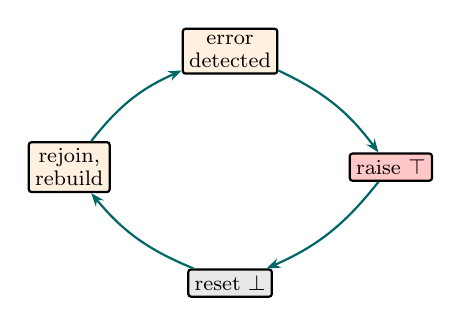
\begin{tikzpicture}[scale=0.95,transform shape,
  box/.style={draw,thick,rounded corners=1pt,fill=orange!12,
              font=\fontsize{7.6}{8.8}\selectfont,inner sep=2.4pt,align=center}]
  \node[box] (d) at (0, 1.55)  {error\\ detected};
  \node[box,fill=red!22]  (e) at ( 2.15, 0) {raise $\top$};
  \node[box,fill=gray!18] (r) at ( 0,-1.55) {reset $\bot$};
  \node[box] (j) at (-2.15, 0) {rejoin,\\ rebuild};
  \draw[garr] (d) to[bend left=14] (e);
  \draw[garr] (e) to[bend left=14] (r);
  \draw[garr] (r) to[bend left=14] (j);
  \draw[garr] (j) to[bend left=14] (d);
\end{tikzpicture}
\par\vspace{1mm}
{\captionfont the self-stabilizing loop}
\end{column}
\end{columns}
\end{frame}

% ==========================================================================
% 11 -- CONCLUSION
% ==========================================================================
\begin{frame}{Conclusion}
\bodyfont
\begin{itemize}\setlength\itemsep{4pt}
\item \textbf{A first:} constant-space, deterministic, self-stabilizing BFS
  \begin{itemize}\setlength\itemsep{1pt}
  \item $O(1)$ bits --- without global parameters
  \end{itemize}
\item \textbf{Key idea:} a token stream with a bounded lifespan
  \begin{itemize}\setlength\itemsep{1pt}
  \item breaks cycles, rebuilds the levels
  \end{itemize}
\item \textbf{Future work:}
  \begin{itemize}\setlength\itemsep{1pt}
  \item asynchronous schedulers: the token proof fails
  \item a polynomial time bound instead of $O(2^{\varepsilon})$
  \end{itemize}
\end{itemize}
\end{frame}

% ==========================================================================
% 12 -- THANK YOU
% ==========================================================================
\begin{frame}[plain]
\vfill
\begin{center}
  {\Huge\bfseries Thank you}
\end{center}
\vfill
\end{frame}

\end{document}
